\documentclass{standalone}
\usepackage{tikz}
\begin{document}
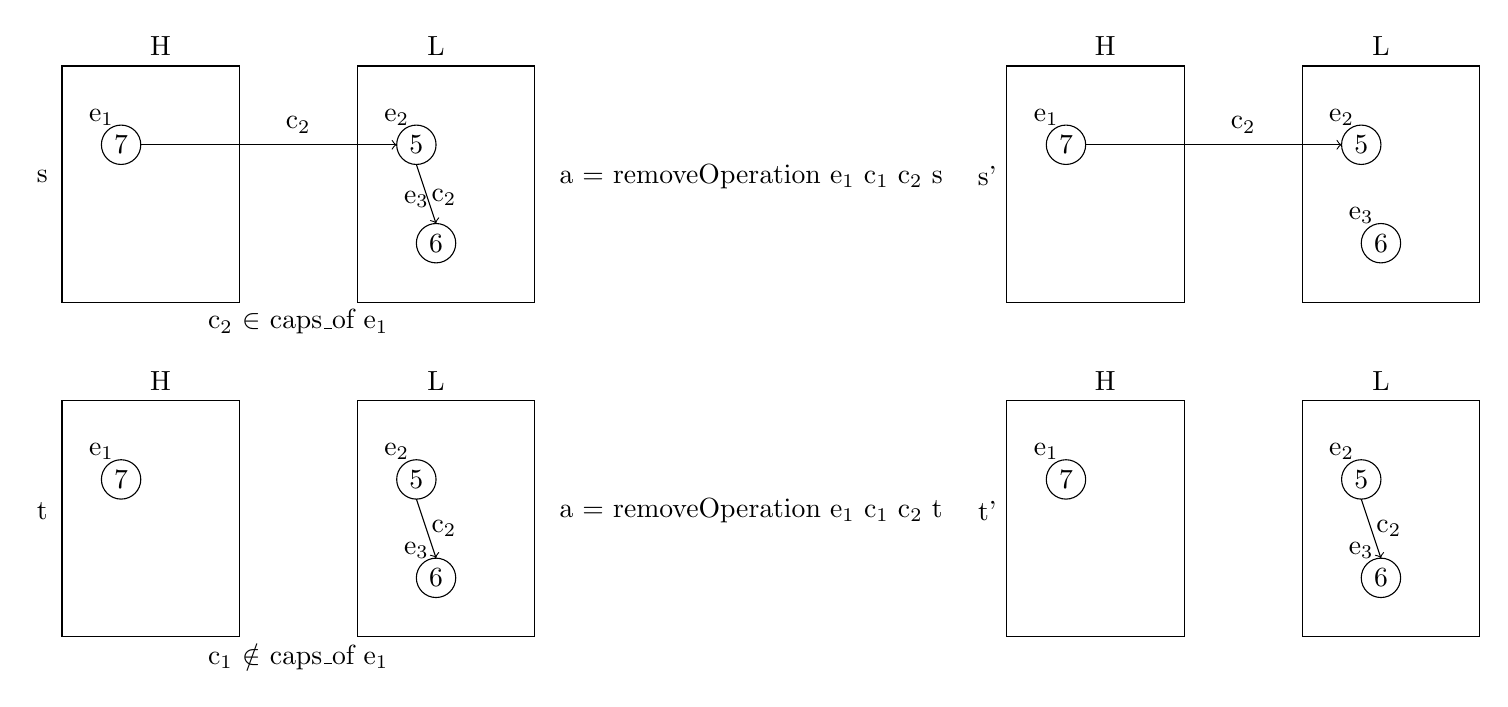
\begin{tikzpicture}
\node at (0,1.6) {t};
\node at (1.5,3.25) {H};
\draw [black] (0.25,0) rectangle (2.5,3);
\draw [black] (4,0) rectangle (6.25,3);
\draw [black] (1,2) circle [radius=0.25] node {7};
\node at (0.75,2.35) {e$_1$};
\node at (5,3.25) {L};
\draw [black] (4.75,2) circle [radius=0.25] node {5};
\node at (4.5,2.35) {e$_2$};
\draw [black] (5,0.75) circle [radius=0.25] node {6};
\node at (4.75,1.1) {e$_3$};
\draw [->, black] (4.75,1.75) -- (5,1);
\node at (5.1,1.375) {c$_2$};
\node at (3.25,-0.25) {c$_1$ $\notin$ caps$\_$of e$_1$};
\node at (9,1.6) {a = removeOperation e$_1$ c$_1$ c$_2$ t};
\node at (12,1.6) {t'};
\node at (13.5,3.25) {H};
\draw [black] (12.25,0) rectangle (14.5,3);
\draw [black] (16,0) rectangle (18.25,3);
\draw [black] (13,2) circle [radius=0.25] node {7};
\node at (12.75,2.35) {e$_1$};
\node at (17,3.25) {L};
\draw [black] (16.75,2) circle [radius=0.25] node {5};
\node at (16.5,2.35) {e$_2$};
\draw [black] (17,0.75) circle [radius=0.25] node {6};
\node at (16.75,1.1) {e$_3$};
\draw [->, black] (16.75,1.75) -- (17,1);
\node at (17.1,1.375) {c$_2$};

\node at (0,5.85) {s};
\node at (1.5,7.5) {H};
\draw [black] (0.25,4.25) rectangle (2.5,7.25);
\draw [black] (4,4.25) rectangle (6.25,7.25);
\draw [black] (1,6.25) circle [radius=0.25] node {7};
\node at (0.75,6.6) {e$_1$};
\node at (5,7.5) {L};
\draw [->, black] (1.25,6.25) -- (4.5,6.25);
\node at (3.25,6.5) {c$_2$};
\draw [black] (4.75,6.25) circle [radius=0.25] node {5};
\node at (4.5,6.6) {e$_2$};
\draw [black] (5,5) circle [radius=0.25] node {6};
\node at (4.75,5.55) {e$_3$};
\draw [->, black] (4.75,6) -- (5,5.25);
\node at (5.1,5.58) {c$_2$};
\node at (3.25,4) {c$_2$ $\in$ caps$\_$of e$_1$};
\node at (9,5.85) {a = removeOperation e$_1$ c$_1$ c$_2$ s};
\node at (12,5.85) {s'};
\node at (13.5,7.5) {H};
\draw [black] (12.25,4.25) rectangle (14.5,7.25);
\draw [black] (16,4.25) rectangle (18.25,7.25);
\draw [black] (13,6.25) circle [radius=0.25] node {7};
\node at (12.75,6.6) {e$_1$};
\node at (17,7.5) {L};
\draw [->, black] (13.25,6.25) -- (16.5,6.25);
\node at (15.25,6.5) {c$_2$};
\draw [black] (16.75,6.25) circle [radius=0.25] node {5};
\node at (16.5,6.6) {e$_2$};
\draw [black] (17,5) circle [radius=0.25] node {6};
\node at (16.75,5.35) {e$_3$};
\end{tikzpicture}
\end{document}
